\documentclass{standalone}
\usepackage{tikz}
\usepackage{amssymb}
\usepackage{fontspec}
\setmainfont{Charis SIL}
\usetikzlibrary{automata, positioning}
\begin{document} 
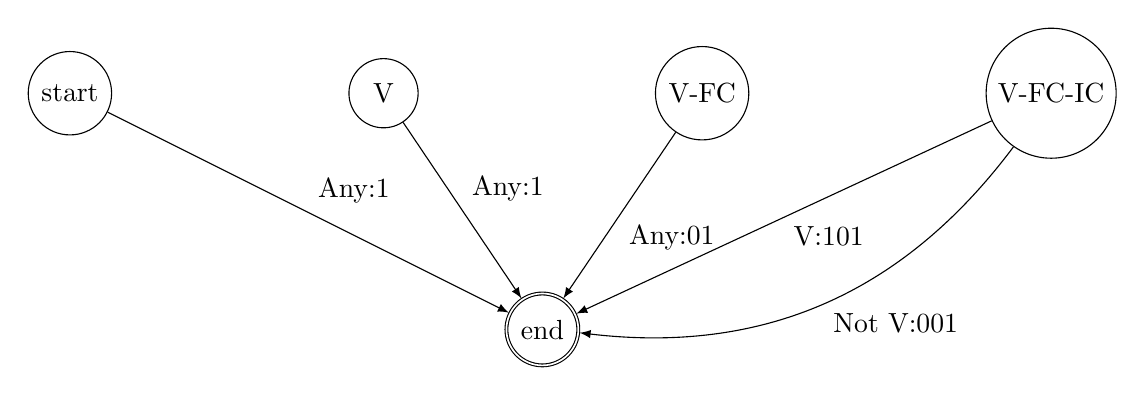
\begin{tikzpicture}[node distance=3cm, auto, every loop/.style={-latex}, every initial by arrow/.style = {-latex}]
\node (q0) [state] {start};
\node (q1) [state, right = of q0] {V};
\node (q2) [state, right = of q1] {V-FC};
\node (q3) [state, right = of q2] {V-FC-IC};
\node (q4) [state, accepting] at (6, -3) {end};
\path [-latex]
     (q0) edge node {Any:1} (q4)
     (q1) edge node {Any:1} (q4)
     (q2) edge node {Any:01} (q4)
     (q3) edge node {V:101} (q4)
     (q3) edge [bend left] node {Not V:001} (q4);
\end{tikzpicture}
 
\end{document}
